
\documentclass[10pt, a4paper]{article}
\usepackage[left=3.5cm, right=3.5cm, top=2cm, bottom=3cm]{geometry}

\usepackage{math_config}
\usepackage{default_config}

\graphicspath{{../figures/}}

\addtolength{\parskip}{\baselineskip}
\parindent 0pt

\begin{document}

%\vspace*{0.2in}
% Title must be 250 characters or less.
\begin{flushleft}
{\Large
\textbf\newline{\textbf{Supplementary Materials} -- Nonrandom connectivity in local cortical circuits from anisotropic axon morphology} % Please use "title case" (capitalize all terms in the title except conjunctions, prepositions, and articles).
}
\newline
% Insert author names, affiliations and corresponding author email (do not include titles, positions, or degrees).
\\[0.1cm]
Felix Z.~Hoffmann, Stefan Rotter \hfill hoffmann@fias.uni-frankfurt.de

%% Felix Z.~Hoffmann, %\textsuperscript{1,2*},
%% Stefan Rotter%\textsuperscript{1,3}
%% \\
%% \bigskip
%% \textbf{1} Bernstein Center Freiburg, Freiburg, Germany
%% \\
%% \textbf{2} Frankfurt Institute for Advanced Studies, Johann Wolfgang Goethe University, Frankfurt am Main, Germany
%% \\
%% \textbf{3} Faculty of Biology, University of Freiburg, Freiburg,
%% Germany
%% \medskip

% Insert additional author notes using the symbols described below. Insert symbol callouts after author names as necessary.
% 
% Remove or comment out the author notes below if they aren't used.

% Use the asterisk to denote corresponding authorship and provide email address in note below.


\end{flushleft}


%\section{Anisotropic random network}

\vspace{0.4cm}

\subsection{Anisotropic network model -- formal definition}
\label{sec:aniso_model}

The anisotropic network model can be formally defined as a random
graph model, in which a realization of the random process results in a
geometric directed graph with a special mode of connectivity. For a
reference on directed graphs see for example \textcite{Bang-Jensen2002}.

\begin{definition*}
  Let $n \in \mathbb{N}$ and $w > 0$. An \textit{anisotropic geometric
    graph} $G_{n,w}$ consists of a tuple $(G,\Phi,a)$, of a simple
  directed graph $G$ with $|V(G)|=n$ vertices and the maps
  $\Phi:V(G)\to[0,1]^2$ and $a:V(G)\to[0,2\pi)$, such that for every
  pair of non-identical vertices $v,v' \in V(G)$ an edge $e\in E(G)$
  from $v$ to $v'$ exists if and only if the inequalities for scalar
  products
  \[
    R_{-a(v)}\left(\Phi(v')-\Phi(v)\right)\hat{e}_x \geq 0 
      \quad \mathrm{and} \quad
    \abs{R_{-a(v)}\left(\Phi(v')-\Phi(v)\right)\hat{e}_y} 
      \leq \frac{w}{2}
  \]
  hold. Here $R_{\varphi}$ is the rotation matrix of angle $\varphi$
  in the Cartesian plane,
  \[
   R_{\varphi} =  \begin{pmatrix}
      \cos \varphi & -\sin \varphi \\  
      \sin \varphi & \cos \varphi \\
    \end{pmatrix},
  \]
  and $\hat{e}_x = (1,0)$, $\hat{e}_y = (0,1)$ are the standard
  unit vectors. % ?? Alpha or A??
  % for $y=A_{\alpha(v)}(v'-v)$ the identities $y\hat{e}_x > 0$
  % and $\abs{y \hat{e}_y} \le \frac{w}{2}$ hold.
\end{definition*}

The anisotropic random graph model is then giving the probability
distribution over the set of anisotropic random graphs by describing a
random process generating such graph.

\begin{definition*}
  Let $n \in \mathbb{N}$ and $w > 0$. The \textit{anisotropic random
    graph model} $G(n,w)$ is a probability space over the set of
  anisotropic geometric graphs with a probability distribution induced
  by the following process: Let $G$ be an empty graph with $n$
  vertices. Assign randomly and uniformly to every vertex $v \in V(G)$
  a position $\Phi(v) \in [0,1]^2$ and axonal orientation
  $0\leq a(v) < 2\pi$. Then add edges such that $(G,\Phi,a)$ is an
  anisotropic geometric graph $G_{n,w}$.
\end{definition*}


We here limited the surface to be the unit square. However, as only
the ratio between $w$ and the side length of the square $E$ determines
connectivity, this doesn't provide a real limitation as $w$ can always
be scaled appropriately to obtain equivalent graphs.



\bigskip

\subsection{Anisotropic network -- Distance-dependent connection probability}

The formal definition of anisotropic graphs in \ref{sec:aniso_model}
allows us for calculation of the distance-dependent connection
probabilities in the network model.

\begin{theorem_w} \label{theorem:distance_prof} Let $G_{n,w} = (G,\Phi,
  a)$ be an anisotropic random graph. Define $C:[0,\sqrt{2}] \to
  [0,1]$ as the distance-dependent connection probability profile of
  $(G,\Phi)$, that is such that $C(x)$ is the probability that for a
  vertex pair $(v,v') \in V(G)^2\setminus\Delta_{V(G)}$ in distance $x
  = \norm{\Phi(v)-\Phi(v')}$ the vertex $v$ projects to vertex
  $v'$. Then
  \[
    C(x) = \begin{cases}%
             \frac{1}{2} & \mathrm{for} \,\, x\le w/2 \\
             \frac{1}{\pi}
             \operatorname{arcsin}\left(\frac{w}{2x}\right) &
             \mathrm{for} \,\, x >  w/2. %
           \end{cases}
  \]
\end{theorem_w} 

\begin{proof}
  Let $v,v'$ be a pair of vertices in $V(G)^2 \setminus \Delta_{V(G)}$
  in Euclidean distance $x$ of each other. The vector difference
  $\Phi(v')-\Phi(v)$ may then be written as $x e^{i\theta}$, with $0
  \leq \theta < 2\pi$. We have 
  \[
    R_{-\alpha(v)} xe^{i\theta} = xe^{i(\theta - \alpha(v))}.
  \]
  Only for suitable combination of $\theta$ and $\alpha(v)$ an edge
  from $v$ to $v'$ exists. Assuming $\alpha(v)$ fixed, we calculate
  the probability of connection depending on the random choice of
  $\theta$. We can assume $\alpha(v) = 0$, otherwise the same argument
  holds for $\theta' = \theta - \alpha(v)$.

  From the definition of the anisotropic random graph we obtain the
  necessary and sufficient conditions
  \[
   x \cos \theta \geq 0 \quad \mathrm{and} \quad \abs{x\sin \theta}
  \leq \frac{w}{2}.
  \]
  Choosing uniformly at random $\theta$ in the range of $[0,2\pi)$,
  the first condition is satisfied with a probability of
  $\frac{1}{2}$. Consider for the second condition $\theta \in
  [0,\pi)$. We have 
  \[ 
  \sin \theta \leq \frac{w}{2x},
  \]
  and for $x \leq \frac{w}{2}$ the inequality holds for all $\theta$
  by definition of $\sin \theta$. In the case of $x > \frac{w}{2}$, we
  note that for the first condition to hold $\theta$ must already be in
  $[0,\frac{\pi}{2})$ and can thus write the second condition $\theta$ as
  \[
    \theta \leq \operatorname{arcsin}\frac{w}{2x},
  \]
  yielding $C(x)$ by combining the considerations above and using the
  symmetry of sine for $\theta$ in the third and fourth quadrant.
  % 
\end{proof}


\vspace{1.6cm}
\addtocounter{subsection}{1}
\begin{figure}[h!] 
  \centering 
  \includegraphics[width=0.65\textwidth]{%
    SI_geomtr-prb/SI_geomtr-prb.pdf}%
  \caption{\textbf{Illustration of the proof} Distance-dependent
    connectivity profile $C(x)$ in an anisotropic geometric graph
    calculated from geometric dependencies. \textbf{A}: In the case of
    $x\leq \nicefrac{w}{2}$, target $v'$ may be located anywhere on
    the shown semicircle and therefore receives input from $v$ with
    probability $\nicefrac{1}{2}$. \textbf{B}: For
    $x > \nicefrac{w}{2}$, suitable positions for target $v'$ are
    dependent on $x$. The geometric relation
    $\sin \theta = \nicefrac{w}{2x}$ leads to the distance-dependent
    connectivity profile as described above.}
  \label{fig:xx_geomtr_prb}
\end{figure}



\clearpage
\newpage

%% \section{Rewiring algorithm}

\subsection*{Choice of rewiring margin $\varepsilon$}

The margin $\varepsilon$ of the rewiring algorithm determines the number of new targets available for a single to be rewired edge. The higher $\varepsilon$, the more targets are available (Fig.~\ref{fig:rew-ddcp-ef}A). To rewire effectively, $\varepsilon$ should be as large as possible. Similarly, the larger $\varepsilon$ the less likely it is for the algorithm to not be able to add the edge back into the graph without creating a parallel edge (Fig.~\ref{fig:rew-ddcp-ef}B). However, to maintain the relative distribution of connected targets at any given distance in the rewired graph $\varepsilon$ should be small (Fig.~\ref{fig:rew-ddcp-ef}C). In our study we chose $\varepsilon/E = 0.05$, where $E=296$ is the length of the square network area.


% say how many edges are lost on average for epsilon=0.05

\textit{Article}: The relative width of the rewiring parameter was chosen as $\varepsilon / E = 0.05$ to optimize the balance between (see SI ??).


\begin{figure}[h!]
  \includegraphics[width=\textwidth]{%
    /home/fh/sci/rsc/aniso_netw/pub/plos_cb_16/figures/SI_rew/SI_rew.pdf}
  \caption{\textbf{Determining the rewiring margin $\bm{\varepsilon}$}. For three anisotropic networks ($N=1000, w=??, E= 296 (??)$), the statistics of rewiring algorithm were recorded for different rewiring margins $\varepsilon$.
    %% the number of rewiring targets was recorded for each edge. Error bars show the average standard deviation. $E=296$ (??) is the length of the square network area in all figures.
    \textbf{A} With increasing $\varepsilon$, the average number of available rewiring targets for a single edge increases. The number of rewiring targets was recorded for each edge. Error bars show the average standard deviation across the three networks.
    \textbf{B} Number of edges that couldn't be rewired and are not included in the rewired network decreases with increasing rewiring margin. Error bars show the standard error of the mean.}
  \label{fig:rew-ddcp-ef}
\end{figure}


\clearpage
\newpage

\subsection{Tuning Distance-dependency}\label{sec:tuned_networks}

The discussion in the last section focused on the effect of anisotropy
in connectivity on the occurrence of neuron pair motifs. Could
distance-dependency itself, as imposed by the specific geometry, be a
decisive factor in the distribution of edge counts in neuron pairs?
%% \textcite{Song2005}, as well as \textcite{Perin2011}, report an
%% overrepresentation of reciprocal connections independent from
%% distance-dependent connectivity, opposing the observations made in the
%% last section (\autoref{fig:two_neuron_probs} A). Furthermore, the
%% connectivity profile in the anisotropic graph model, as identified in
%% Section~\ref{sec:distance_connectivity}, follows purely from abstract
%% geometry rather than being motivated by connectivity found in cortical
%% circuits. In an attempt to rectify this and to allow for a more
%% differentiated examination of two neuron connections, in this section
%% we step away from simplistic geometry and \enquote{tune} the
%% anisotropic networks to display a distance-dependent connectivity as
%% reported by Perin et al. by adjusting the width $w(x)$ at any point
%% $x$ along the axon's projection.

%% For this we introduce anisotropic networks tuned to reflect a given
%% distance-dependent connection profile $C(x)$. We are facing the
%% following problem: Given $C(x):[0,\sqrt{2}) \to [0,1]$, find
%% $w:[0,\sqrt{2}) \to [0,\infty)$ such that the probability to have a
%% connection from $v_1$ to $v_2$ for arbitrary vertices $v_1 \neq v_2$
%% in an anisotropic graph $G(n,w)$ with distance $\mathrm{d}(v_1,v_2) =
%% x$ is $C(x)$. The problem is in general highly complex when nothing
%% can be assumed about $C(x)$. We find an approximate solution to the
%% problem considering the following geometric relation:

%% \begin{figure}[htp]
%%   \centering
%%   \makebox{%
%%     \begin{overpic}[height=3.35cm]{%
%%         plots/bed7650b.pdf}
%%     \end{overpic}
%%   }%
%%   \caption{Computing connection probability $C(x)$ from non-constant
%%     $w(x)$}
%%   \label{fig:dpp_wc}
%% \end{figure}

%% From \autoref{fig:dpp_wc} we have the relation  
%% \begin{equation}
%% C\left(\sqrt{x^2+w^2(x)}\right) = \frac{1}{\pi} \operatorname{arctan}
%% \frac{w(x)}{x}. \label{eq:geo_rel}
%% \end{equation} 
%% In order to solve for $w(x)$ we first consider a linear approximation,
%% expanding
%% \[C\left(\sqrt{x^2+w^2(x)}\right) \approx C(x) + \left(\sqrt{x^2+w^2(x)} -
%% x\right) C'(x).\]

%% The resulting transcendental equation
%% \[C(x) + \left(\sqrt{x^2+w^2(x)} -
%% x\right) C'(x) = \frac{1}{\pi} \operatorname{arctan}
%% \frac{w(x)}{x}\]
%% is however still too complex in the context of this work. Instead we
%% propose the approximation $\sqrt{x^2 + w^2(x)} \approx  x$, which
%% inserting into \ref{eq:geo_rel} yiels
%% \begin{equation}
%% C(x) \approx \frac{1}{\pi} \operatorname{arctan} \label{eq:tanapprox}
%% \frac{w(x)}{x}.
%% \end{equation}

%% Under the assumption that $C(x)<\frac{1}{2}$ for all $x$ we obtain the
%% identity
%% \begin{equation}
%%   w(x) = x \tan\left( \pi\, C(x) \right), \label{eq:xtan}
%% \end{equation} 
%% being aware that it only holds as well as
%% approximation~\ref{eq:tanapprox} does. 

%% Here we use relation~\ref{eq:xtan} to generate anisotropic networks
%% reflecting the dis\-tance-de\-pendent connectivity profile as found by
%% \textcite{Perin2011}. For this we finally need to adjust the before
%% arbitrarily determined side length of the network's surface. Perin et
%% al.~mapped connectivity in layer 5 of the rat's somatosensory cortex
%% up to a distance of $\SI{300}{\micro\meter}$. Using this reported
%% distance connectivity to generate anisotropic networks via
%% \ref{eq:xtan}, the chosen side length $s$ determines the networks
%% overall connectivity (\autoref{fig:determine_side_length} A). We
%% determine $s = \SI{296}{\micro\meter}$ to match the overall connection
%% probability of $p = 0.116$ as used before and reported by Song et
%% al.~(\autoref{fig:determine_side_length} B). The obtained value for
%% $s$ is consistent with the slice thickness of \SI{300}{\micro\meter}
%% used in Perin et al.'s experiment.


%% %% \begin{figure}[htp]
%% %%   \centering
%% %%   \makebox{%
%% %%     \begin{overpic}[height=4.05cm]{%
%% %%         plots/6154302f.pdf}
%% %%       \put(85.5,57.0){\small\textbf{A}}
%% %%       %\put(12,5){\small\textbf{A}}
%% %%     \end{overpic}
%% %%     \hfill
%% %%     \begin{overpic}[height=3.955cm]{%
%% %%         plots/ef0e785d.pdf}
%% %%       \put(88.5,58.2){\small\textbf{B}}
%% %%     \end{overpic}
%% %%   }%
%% %%   \captionsetup{skip=7pt}
%% %%   \caption{\textbf{Network side length adjusted to match overall
%% %%       connection probability} Side length of the network's surface
%% %%     determines the overall connection probability in the network when
%% %%     axon width function $w(x)$ is fixed. \textbf{A)} Connection
%% %%     probability declines with rising side length \textbf{B)}
%% %%     Determining side length as $s=\SI{296}{\micro\meter}$ to match $p
%% %%     = 0.116$ as reported by \textcite{Song2005}. (\smtcite{6154302f},
%% %%     \smtcite{ef0e785d})}
%% %%   \label{fig:determine_side_length}
%% %% \end{figure}



%% Having determined the neotwork's side length $s$, we're extending the
%% quiver of generated sample networks for the numerical analysis once
%% more by the \enquote{tuned anisotropic graphs}\index{tuned
%%   anisotropic networks}, in which the axon width $w(x)$ was determined
%% such that the networks reflect Perin's connectivity profile. Analyzing
%% the obtained axon width function we note that $x \gg w(x)$ holds for
%% most $x$, justifying the approximation
%% \[
%%   \sqrt{x^2 + w^2(x)} \approx x
%% \] 
%% \textit{a posteriori} (\autoref{fig:perin_axwidth}). From the 25
%% generated networks overall connection probability is extracted as $p =
%% 0.1160 \pm 0.0006$ (SEM), as expected from the choice of $s$
%% (\smtcite{f11dca65}).



%% % This approximation holds well as long as $x \gg w(x)$. Using the
%% % relation to tune the axon width to produce anisotropic networks with a
%% % distance-dependency as reported by Perin et al., we find that for all $x$ is
%% % strictly greater than $w(x)$  %(\autoref{fig:perin_axwidh


%% \begin{figure}[htp]
%%   \centering
%%   \hspace{0.05cm}
%%   \begin{overpic}[width=0.6\textwidth]{%
%%       plots/d45c02e4.pdf}
%%           \put(69.4,51.5){\small\textbf{A}}
%%   \end{overpic}
%%   \hfill
%%   \begin{overpic}[width=0.35\textwidth]{%
%%       plots/8f0d65e4.pdf}
%%     \put(81,86){%
%%       \fboxsep=2pt\colorbox{white}{\small\textbf{B}}
%%     }
%%   \end{overpic}
%%   \captionsetup{skip=7pt}
%%   \caption{\textbf{Anisotropic network model with tuned axon width
%%       $\mathbf{w(x)}$} \textbf{A)} Resulting axon width function
%%     $w(x)$ from tuning to distance-dependent connection profile as
%%     reported by \textcite{Perin2011}, see also
%%     \autoref{fig:perin_profiles}. Note that $x \gg w(x)$ for most $x$,
%%     supporting approximation~\ref{eq:tanapprox}. \textbf{B)}
%%     Showing for a single neuron (star) connected (red) and unconnected
%%     (gray) neurons in the tuned anisotropic network, revealing
%%     the characteristic axon shape. (\smtcite{d45c02e4}, \smtcite{8f0d65e4})}
%%   \label{fig:perin_axwidth}
%% \end{figure}




%% Overall distance-dependent connection probabilities in the tuned
%% an\-iso\-tro\-pic graphs clearly match the profile of Perin et
%% al.~(\autoref{fig:perin_profiles} A), presenting strongest the
%% argument in support of the chosen approximation. Analyzing two neuron
%% connections \marginpar{revisiting two neuron connections} in the tuned
%% networks, we affirm the findings of the last section. In their
%% experiment, Perin et al.~were able to show an overrepresentation of
%% reciprocal connections at any inter-neuron distance
%% (\autoref{fig:perin_profiles} B-C). Rather than matching these
%% profiles, we find that occurrences of one- and bidirectionally
%% connected pairs in the anisotropic graphs align with probabilities
%% obtained from the distance-dependent overall connection probability
%% $p(x)$ under the assumption of independence (cf. Equation~\ref{eq:pairs}),
%% \begin{equation*}
%%   \label{eq:pairs}
%%   \begin{aligned}%
%%     & \mathbf{P}_{X=1}(x) = 2p(x) \left(1-p(x) \right)    
%%       && \text{single connection,}\\
%%     & \mathbf{P}_{X=2}(x) = p(x)^2        
%%       &&\text{reciprocal connection.}
%%   \end{aligned}%
%% \end{equation*}%
%% \vspace{0.1cm}%
%% Thus, in comparison with Perin et al.'s findings, we find that
%% anisotropy in connectivity cannot account for the overrepresentation
%% in reciprocal connections. While results in
%% Section~\ref{sec:two_neuron} still indicated such an
%% overrepresentation due to distance-dependency, examining the
%% occurrence of two neuron connections at any inter-neuron distance in
%% anisotropic networks, tuned to a distance-dependent connection profile
%% matching experimental findings from cortical circuits, imply complete
%% unrelatedness of anisotropy and two-neuron connection distributions.

%% \begin{figure}[htp]
%%   \centering
%%   \makebox{%
%%     \begin{overpic}[width=0.5\textwidth]{%
%%         plots/875505b0_overall.pdf}
%%       \put(28,19){\small\textbf{A}}
%%     \end{overpic}
%%     \hfill
%%     \begin{overpic}[width=0.5\textwidth]{%
%%         plots/875505b0_single.pdf}
%%       \put(28,19){\small\textbf{B}}
%%     \end{overpic}
%%   }%
%%   \vspace{-0.6cm}
%%   \makebox{%
%%     \begin{overpic}[width=0.5\textwidth]{%
%%         plots/875505b0_recip.pdf}
%%        \put(28,19){\small\textbf{C}}
%%     \end{overpic}
%%     \vspace{-1cm}
%%     \includegraphics[width=0.5\textwidth]{%
%%       img/tuned_legend.pdf}   
%%   }%
%%   \captionsetup{skip=7pt}
%%   \caption{\textbf{Distance-independent overrepresentation of
%%       reciprocal connections} Comparison of occurrences of one- and
%%     bidirectionally connected neuron pairs in the tuned anisotropic
%%     networks (gray) with profiles found by Perin et al.~(red), shows
%%     that overrepresentation of bidirectional pairs is
%%     distance-independent and not connected to anisotropy.  \textbf{A)}
%%     Overall connection probability in the tuned anisotropic networks
%%     was successfully adjusted to reflect connection probability found
%%     by Perin et al. \textbf{B)-C)} Showing in blue the probabilities
%%     to obtain a neuron pair motif (single edge in B, two edges in C)
%%     calculated under independence assumption from the overall
%%     probability from A), we find that counts in the tuned anisotropic
%%     networks (gray) match the independence assumption and do
%%     \textit{not} show the overrepresentation present in Perin et al.'s
%%     experiment. (\smtcite{875505b0})}
%%   \label{fig:perin_profiles}
%% \end{figure}






\bigskip

\subsection{Tuning anisotropic networks to specific distance-dependent
  connection probabilities}
\label{sec:tuned_networks}


In tuned anisotropic graphs, the form of the width function $w(x)$
determines the distance-dependent connection probability $C(x)$ in the
network. Here, we are interested in determining $w(x)$ such that
$C(x)$ matches the probabilities as found by \textcite{Perin2011}.

In general, let $C(x): [0,\sqrt{2}) \to [0,1]$ be a distance-dependent
  connection probability on the unit square. From

  \begin{figure}[h!]
    \centering
    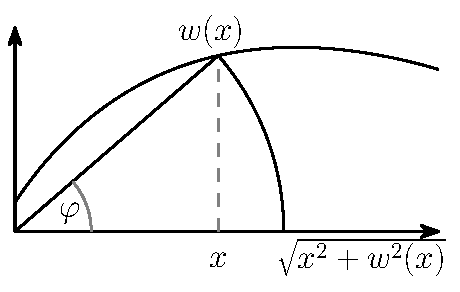
\includegraphics[width=0.35\textwidth]{%
    img/distance-dependent-relation-in-tuned-networks.pdf} %
  \end{figure}

 we obtain the relation
%
\begin{align}
C\left(\sqrt{x^2+w^2(x)}\right) = \frac{1}{\pi} \operatorname{arctan}
\frac{w(x)}{x}. \label{eq:geo_rel}
\end{align}
%
In order to solve for $w(x)$ we approximate $\sqrt{x^2 + w^2(x)}
\approx x$, which inserting into \eqref{eq:geo_rel} yields
\begin{equation}
C(x) \approx \frac{1}{\pi} \operatorname{arctan} \label{eq:tanapprox}
\frac{w(x)}{x}.
\end{equation}
%
Under the assumption that $C(x)<\frac{1}{2}$ for all $x \in
[0,\sqrt{2})$ we obtain the identity
\begin{equation}
  w(x) = x \tan\left( \pi\, C(x) \right). \label{eq:xtan}
\end{equation} 
%
With the distance-dependent connection probabilities
\begin{align}
C(x) = -0.00142\, \left(0.00276 + x^{-0.945}\right)^{-1} + 0.23079
\end{align}
%
from \textcite{Perin2011} we . However, since here $x$ was measured in
\SI{}{\micro\meter}

Here we use relation~\ref{eq:xtan} to generate anisotropic networks
reflecting the dis\-tance-de\-pendent connectivity profile as found by
\textcite{Perin2011}. For this we finally need to adjust the before
arbitrarily determined side length of the network's surface. Perin et
al.~mapped connectivity in layer 5 of the rat's somatosensory cortex
up to a distance of $\SI{300}{\micro\meter}$. Using this reported
distance connectivity to generate anisotropic networks via
\ref{eq:xtan}, the chosen side length $s$ determines the networks
overall connectivity (\autoref{fig:determine_side_length} A). We
determine $s = \SI{296}{\micro\meter}$ to match the overall connection
probability of $p = 0.116$ as used before and reported by Song et
al.~(\autoref{fig:determine_side_length} B). The obtained value for
$s$ is consistent with the slice thickness of \SI{300}{\micro\meter}
used in Perin et al.'s experiment.


%% %% \begin{figure}[htp]
%% %%   \centering
%% %%   \makebox{%
%% %%     \begin{overpic}[height=4.05cm]{%
%% %%         plots/6154302f.pdf}
%% %%       \put(85.5,57.0){\small\textbf{A}}
%% %%       %\put(12,5){\small\textbf{A}}
%% %%     \end{overpic}
%% %%     \hfill
%% %%     \begin{overpic}[height=3.955cm]{%
%% %%         plots/ef0e785d.pdf}
%% %%       \put(88.5,58.2){\small\textbf{B}}
%% %%     \end{overpic}
%% %%   }%
%% %%   \captionsetup{skip=7pt}
%% %%   \caption{\textbf{Network side length adjusted to match overall
%% %%       connection probability} Side length of the network's surface
%% %%     determines the overall connection probability in the network when
%% %%     axon width function $w(x)$ is fixed. \textbf{A)} Connection
%% %%     probability declines with rising side length \textbf{B)}
%% %%     Determining side length as $s=\SI{296}{\micro\meter}$ to match $p
%% %%     = 0.116$ as reported by \textcite{Song2005}. (\smtcite{6154302f},
%% %%     \smtcite{ef0e785d})}
%% %%   \label{fig:determine_side_length}
%% %% \end{figure}



%% Having determined the neotwork's side length $s$, we're extending the
%% quiver of generated sample networks for the numerical analysis once
%% more by the \enquote{tuned anisotropic graphs}\index{tuned
%%   anisotropic networks}, in which the axon width $w(x)$ was determined
%% such that the networks reflect Perin's connectivity profile. Analyzing
%% the obtained axon width function we note that $x \gg w(x)$ holds for
%% most $x$, justifying the approximation
%% \[
%%   \sqrt{x^2 + w^2(x)} \approx x
%% \] 
%% \textit{a posteriori} (\autoref{fig:perin_axwidth}). From the 25
%% generated networks overall connection probability is extracted as $p =
%% 0.1160 \pm 0.0006$ (SEM), as expected from the choice of $s$
%% (\smtcite{f11dca65}).



%% % This approximation holds well as long as $x \gg w(x)$. Using the
%% % relation to tune the axon width to produce anisotropic networks with a
%% % distance-dependency as reported by Perin et al., we find that for all $x$ is
%% % strictly greater than $w(x)$  %(\autoref{fig:perin_axwidh


%% \begin{figure}[htp]
%%   \centering
%%   \hspace{0.05cm}
%%   \begin{overpic}[width=0.6\textwidth]{%
%%       plots/d45c02e4.pdf}
%%           \put(69.4,51.5){\small\textbf{A}}
%%   \end{overpic}
%%   \hfill
%%   \begin{overpic}[width=0.35\textwidth]{%
%%       plots/8f0d65e4.pdf}
%%     \put(81,86){%
%%       \fboxsep=2pt\colorbox{white}{\small\textbf{B}}
%%     }
%%   \end{overpic}
%%   \captionsetup{skip=7pt}
%%   \caption{\textbf{Anisotropic network model with tuned axon width
%%       $\mathbf{w(x)}$} \textbf{A)} Resulting axon width function
%%     $w(x)$ from tuning to distance-dependent connection profile as
%%     reported by \textcite{Perin2011}, see also
%%     \autoref{fig:perin_profiles}. Note that $x \gg w(x)$ for most $x$,
%%     supporting approximation~\ref{eq:tanapprox}. \textbf{B)}
%%     Showing for a single neuron (star) connected (red) and unconnected
%%     (gray) neurons in the tuned anisotropic network, revealing
%%     the characteristic axon shape. (\smtcite{d45c02e4}, \smtcite{8f0d65e4})}
%%   \label{fig:perin_axwidth}
%% \end{figure}




%% Overall distance-dependent connection probabilities in the tuned
%% an\-iso\-tro\-pic graphs clearly match the profile of Perin et
%% al.~(\autoref{fig:perin_profiles} A), presenting strongest the
%% argument in support of the chosen approximation. Analyzing two neuron
%% connections \marginpar{revisiting two neuron connections} in the tuned
%% networks, we affirm the findings of the last section. In their
%% experiment, Perin et al.~were able to show an overrepresentation of
%% reciprocal connections at any inter-neuron distance
%% (\autoref{fig:perin_profiles} B-C). Rather than matching these
%% profiles, we find that occurrences of one- and bidirectionally
%% connected pairs in the anisotropic graphs align with probabilities
%% obtained from the distance-dependent overall connection probability
%% $p(x)$ under the assumption of independence (cf. Equation~\ref{eq:pairs}),
%% \begin{equation*}
%%   \label{eq:pairs}
%%   \begin{aligned}%
%%     & \mathbf{P}_{X=1}(x) = 2p(x) \left(1-p(x) \right)    
%%       && \text{single connection,}\\
%%     & \mathbf{P}_{X=2}(x) = p(x)^2        
%%       &&\text{reciprocal connection.}
%%   \end{aligned}%
%% \end{equation*}%
%% \vspace{0.1cm}%
%% Thus, in comparison with Perin et al.'s findings, we find that
%% anisotropy in connectivity cannot account for the overrepresentation
%% in reciprocal connections. While results in
%% Section~\ref{sec:two_neuron} still indicated such an
%% overrepresentation due to distance-dependency, examining the
%% occurrence of two neuron connections at any inter-neuron distance in
%% anisotropic networks, tuned to a distance-dependent connection profile
%% matching experimental findings from cortical circuits, imply complete
%% unrelatedness of anisotropy and two-neuron connection distributions.

%% \begin{figure}[htp]
%%   \centering
%%   \makebox{%
%%     \begin{overpic}[width=0.5\textwidth]{%
%%         plots/875505b0_overall.pdf}
%%       \put(28,19){\small\textbf{A}}
%%     \end{overpic}
%%     \hfill
%%     \begin{overpic}[width=0.5\textwidth]{%
%%         plots/875505b0_single.pdf}
%%       \put(28,19){\small\textbf{B}}
%%     \end{overpic}
%%   }%
%%   \vspace{-0.6cm}
%%   \makebox{%
%%     \begin{overpic}[width=0.5\textwidth]{%
%%         plots/875505b0_recip.pdf}
%%        \put(28,19){\small\textbf{C}}
%%     \end{overpic}
%%     \vspace{-1cm}
%%     \includegraphics[width=0.5\textwidth]{%
%%       img/tuned_legend.pdf}   
%%   }%
%%   \captionsetup{skip=7pt}
%%   \caption{\textbf{Distance-independent overrepresentation of
%%       reciprocal connections} Comparison of occurrences of one- and
%%     bidirectionally connected neuron pairs in the tuned anisotropic
%%     networks (gray) with profiles found by Perin et al.~(red), shows
%%     that overrepresentation of bidirectional pairs is
%%     distance-independent and not connected to anisotropy.  \textbf{A)}
%%     Overall connection probability in the tuned anisotropic networks
%%     was successfully adjusted to reflect connection probability found
%%     by Perin et al. \textbf{B)-C)} Showing in blue the probabilities
%%     to obtain a neuron pair motif (single edge in B, two edges in C)
%%     calculated under independence assumption from the overall
%%     probability from A), we find that counts in the tuned anisotropic
%%     networks (gray) match the independence assumption and do
%%     \textit{not} show the overrepresentation present in Perin et al.'s
%%     experiment. (\smtcite{875505b0})}
%%   \label{fig:perin_profiles}
%% \end{figure}





 %%%%% ------------------------------


   
  
%% For this we introduce anisotropic networks tuned to reflect a given
%% distance-dependent connection profile $C(x)$. We are facing the
%% following problem: Given $C(x):[0,\sqrt{2}) \to [0,1]$, find
%% $w:[0,\sqrt{2}) \to [0,\infty)$ such that the probability to have a
%% connection from $v_1$ to $v_2$ for arbitrary vertices $v_1 \neq v_2$
%% in an anisotropic graph $G(n,w)$ with distance $\mathrm{d}(v_1,v_2) =
%% x$ is $C(x)$. The problem is in general highly complex when nothing
%% can be assumed about $C(x)$. We find an approximate solution to the
%% problem considering the following geometric relation:

%% \begin{figure}[htp]
%%   \centering
%%   \makebox{%
%%     \begin{overpic}[height=3.35cm]{%
%%         plots/bed7650b.pdf}
%%     \end{overpic}
%%   }%
%%   \caption{Computing connection probability $C(x)$ from non-constant
%%     $w(x)$}
%%   \label{fig:dpp_wc}
%% \end{figure}



\clearpage
\newpage

%% \section{Network motifs of three neurons}
\subsection{Three-neuron motif statistics}
\label{sec:3motif_stat}

There are 16 %
% %------------------------------------
% \footnote{%
%   There are 16 non-isomorphic simple directed graphs with 3
%   nodes. Three of those graphs are unconnected \parencite[cf. ][%
%   N. J. A. Sloane. The On-Line Encyclopedia of Integer Sequences,
%   http://oeis.org. Sequence
%   \href{http://oeis.org/A000273}{A000273}]{Davis1953}.%
% } %
% %-------------------------------------
non-isomorphic 3-motifs %?? by the strict definition 1-3 are not
                        %motifs
in simple directed graphs. In accordance with the study of
\textcite{Song2005}, the patterns were labeled 1 to 16
(Fig.~\ref{MAIN-fig:3_motifs}). Assuming independence, the expected
distribution for the random variable $X$, that maps three random
vertices $v_1 \neq v_2 \neq v_3$ in a graph $G$ to the
$n \in \{1,2,\dots,16\}$, labeling the isomorphism class of the full
subgraph with vertex set $\{v_1,v_2,v_3\}$ in $G$ as above, can be
obtained from pair connection statistics. In anisotropic networks we
found that the probabilities of occurrence are
\begin{align*} 
  p_u & = 0.791336     &&\text{for unconnected pairs,}     \\
  p_s & = 0.184151     &&\text{for pairs with a single connection and} \\
  p_r & = 0.024513     &&\text{for reciprocally connected pairs.}
\end{align*}
We denote with $p_{\bar{s}} = p_s/2$ the probability to find a single
connection from $v_1$ in $v_2$ in a vertex pair $(v_1,v_2)$. The
probability of occurrence of the motif with label \enquote{8} is then
the product of the probabilities of it constituents multiplied with a
factor
\[
  \mathbf{P}(X=8) = 6\, p_{u} p_{\bar{s}} p_{r},
\]
where the factor 6 is determined by the number of different
\textit{labeled} graphs belonging to the isomorphism class. The
distribution of $X$ for the remaining motifs is given by \\
%
\smallskip
%
\begin{minipage}{\linewidth}
  \begin{minipage}[c]{0.32\textwidth}
    \begin{align*}
      \mathbf{P}(X=1) &    =   p_u^3  \\
      \mathbf{P}(X=2) &    =   6 p_u p_u p_{\bar{s}}\\
      \mathbf{P}(X=3) &    =   3 p_u p_u p_r\\
      \mathbf{P}(X=4) &    =   3 p_{\bar{s}}^2 p_u\\
      \mathbf{P}(X=5) &    =   3 p_{\bar{s}}^2 p_u\\
    \end{align*}
  \end{minipage}%
  \begin{minipage}[c]{0.32\textwidth}
    \begin{align*}
      \mathbf{P}(X=\,\,\,6) &    =   6 p_{\bar{s}}^2 p_u\\
      \mathbf{P}(X=\,\,\,7) &    =   6 p_{\bar{s}} p_u p_r\\
      \mathbf{P}(X=\,\,\,9) &    =   3 p_r^2 p_u\\
      \mathbf{P}(X=10) &   =   6 p_{\bar{s}}^3   \\
      \mathbf{P}(X=11) &   =   2 p_{\bar{s}}^3    \\
    \end{align*}
  \end{minipage}%
  \begin{minipage}[c]{0.32\textwidth}
    \begin{align*}
      \mathbf{P}(X=12) &   =   3 p_{\bar{s}}^2 p_r\\
      \mathbf{P}(X=13) &   =   6 p_{\bar{s}}^2 p_r\\
      \mathbf{P}(X=14) &   =   3 p_{\bar{s}}^2 p_r\\
      \mathbf{P}(X=15) &   =   6 p_{\bar{s}} p_r^2\\
      \mathbf{P}(X=16) &   =   p_r^3.\\
    \end{align*}
  \end{minipage}  
\end{minipage}

There are $4^3 = 64$ possible combinations to obtain a three motif
from unconnected, unidirectionally connected (both directions) and
bidirectionally connected pairs. Summing up the coefficients for
motifs 1-16 as above yields exactly this number. It is further
\[\sum_{i=1}^{16} \mathbf{P}(X=i) = (p_u+2p_{\bar{s}}+p_r)^3 = 1,\]
verifying the motif distribution above.


\subsection*{Neuron clustering}


\begin{figure}[h!]
  \includegraphics[width=\textwidth]{%
    /home/fh/sci/rsc/aniso_netw/pub/arxiv18/figures/SI_netclst/SI_netclst_figure.pdf}
  \caption{\textbf{Determining the rewiring margin $\bm{\varepsilon}$}. For three anisotropic networks ($N=1000, w=??, E= 296 (??)$), the statistics of the rewiring algorithm were recorded for different rewiring margins $\varepsilon$.
    %% the number of rewiring targets was recorded for each edge. Error bars show the average standard deviation. $E=296$ (??) is the length of the square network area in all figures.
    \textbf{A}. With increasing $\varepsilon$, the average number of available rewiring targets for a single edge increases. The number of rewiring targets was recorded for each edge and then averaged for every graph. Error bars show the average standard deviation for the number of targets within a network.
    \textbf{B}. Number of edges that couldn't be rewired and are not included in the rewired network decreases with increasing rewiring margin. Error bars show the standard error of the mean. \textbf{C}. Distance-dependent connection probability before (blue) and after rewiring (green). The larger $\varepsilon$, the more the distance-dependent connection probabilities differ in the rewired network from the original profile. For each graph, distances between connected were extracted and binned ($n=100$) and divided by the frequency of the distance occurring in the graph. The lighter areas around the curves represent SEMs across the three networks.}
  \label{fig:nclst}
\end{figure}


\subsection{Common neighbours}



\addtocounter{subsection}{1}
\begin{figure}[h!]
  \includegraphics[width=\textwidth]{%
    /home/fh/sci/rsc/aniso_netw/pub/arxiv18/figures/common_inputs/commom_inputs.pdf}
  \caption{\textbf{Determining the rewiring margin $\bm{\varepsilon}$}. For three anisotropic networks ($N=1000, w=??, E= 296 (??)$), the statistics of the rewiring algorithm were recorded for different rewiring margins $\varepsilon$.
    \textbf{A}. With increasing $\varepsilon$, the average number of available rewiring targets for a single edge increases. The number of rewiring targets was recorded for each edge and then averaged for every graph. Error bars show the average standard deviation for the number of targets within a network.
    \textbf{B}. Number of edges that couldn't be rewired and are not included in the rewired network decreases with increasing rewiring margin. Error bars show the standard error of the mean. \textbf{C}. Distance-dependent connection probability before (blue) and after rewiring (green). The larger $\varepsilon$, the more the distance-dependent connection probabilities differ in the rewired network from the original profile. For each graph, distances between connected were extracted and binned ($n=100$) and divided by the frequency of the distance occurring in the graph. The lighter areas around the curves represent SEMs across the three networks.}
  \label{fig:nclst}
\end{figure}


\addtocounter{subsection}{1}
\begin{figure}[h!]
  \includegraphics[width=\textwidth]{%
/home/fh/sci/rsc/aniso_netw/pub/arxiv18/figures/common_inputs/common_outputs.pdf}  \caption{\textbf{Determining the rewiring margin $\bm{\varepsilon}$}. For three anisotropic networks ($N=1000, w=??, E= 296 (??)$), the statistics of the rewiring algorithm were recorded for different rewiring margins $\varepsilon$.
    \textbf{A}. With increasing $\varepsilon$, the average number of available rewiring targets for a single edge increases. The number of rewiring targets was recorded for each edge and then averaged for every graph. Error bars show the average standard deviation for the number of targets within a network.
    \textbf{B}. Number of edges that couldn't be rewired and are not included in the rewired network decreases with increasing rewiring margin. Error bars show the standard error of the mean. \textbf{C}. Distance-dependent connection probability before (blue) and after rewiring (green). The larger $\varepsilon$, the more the distance-dependent connection probabilities differ in the rewired network from the original profile. For each graph, distances between connected were extracted and binned ($n=100$) and divided by the frequency of the distance occurring in the graph. The lighter areas around the curves represent SEMs across the three networks.}
  \label{fig:nclst}
\end{figure}




\clearpage
\newpage

\printbibliography

\end{document}

